\section{Controller}

%Snake is only fun if you can actually control the snake. The STK500 have 8 switches which could have been used, but they are both hard to press precisely and fast. They are also clunky as you would have to either hold the whole board or lean over it. To combat this we added a old NES Controller from the Nintendo Entertainment System. It's a simple controller, also with 8 buttons. It uses a TC4021B 8-Stage Static Shift Register and uses its parallel in / serial out operations to transfer which buttons are pushed.

We are using the NES Controller to control the snake. It's a simple controller, also with 8 buttons. The controller uses a TC4021B 8-Stage Static Shift Register. The TC4021B has five connections available to us\cite{toshiba:tc4021b}:
\begin{itemize}
\item \texttt{Clock}
\item \texttt{Latch}
\item \texttt{Data}
\item \texttt{VCC}
\item \texttt{GND}
\end{itemize}

The \texttt{VCC} needs to be 5V as 3.3V, referring to the displays requirements, is not enough to drive the TC4021B.

The \texttt{Latch} in the TC4021B is used to shift between parallel mode and serial mode. In parallel mode, the buttons state is continuously latched into the TC4021B. In serial mode, the \texttt{Data} pin has the state of the "current bit", and each time you make a pulse on the \texttt{Clock} pin the bits are shifted.

Therefore you need seven pulses to read the eight bits out. After the seven pulses the Latch needs to be set to high again to get the new inputs as seen in Figure~\ref{fig:controller_cycle}

\begin{figure}
\centering
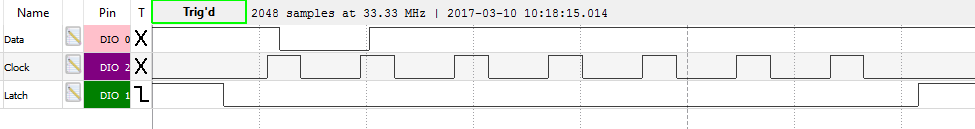
\includegraphics[width=0.9\textwidth]{architecture/controller_cycle}
\caption{A full transmission, where the B buttons is pushed}
\label{fig:controller_cycle}
\end{figure}

The order of the states of the buttons, that are transfered, are found by  trial and error, as there is no official public data sheet for the controller. It's worth noting that the buttons are active LOW. The order are as follows: A, B, Select, Start, Up, Down, Left, Right.

Instead of cutting the cord on the controller, we bought an extension cord. We then mapped the colors of the connections in the extension cord as seen in Figure~\ref{fig:nes}.

\begin{figure}
\centering
\begin{BVerbatim}
         +----> VCC    (yellow)
         |
4 +---------+ 6
 | x  x  o   \
 | o  o  o  o |
3 +-----------+ 0
   |  |  |  |
   |  |  |  +-> GND    (brown)
   |  |  +----> Pulse  (orange)
   |  +-------> Latch  (black)
   +----------> Data   (red)
\end{BVerbatim}
\caption{Layout of cables in the NES Controller extension cord}
\label{fig:nes}
\end{figure}

\subsection{SPI driver}

The SPI interface of the ATMEGA32 is pretty straight forward. There is a few parameters, we need to keep in mind:

\begin{itemize}
\item SPI mode
\item Clock frequency
\item Endianness
\end{itemize}

These properties will have to match the properties defined in the data sheet of the Display. The implementation will be described in Chapter~\ref{cha:implementation}.

\subsection{Controller driver}

To make it easier to read the controller, we a made a simple driver that uses the software SPI driver to read the states of the buttons. As it's a one-way read communication, it simply reads and parses the signal, and set the different button value accordingly.

The implementation will be described in Chapter~\ref{cha:implementation}.

